%%%%%%%%%%%%%%%%%%%%%%%%%%%%%%%%%%%%%
%                                   %
% Compile with XeLaTeX and biber    %
%                                   %
% Questions or comments:            %
%                                   %
% joshua dot mcneill at uga dot edu %
%                                   %
%%%%%%%%%%%%%%%%%%%%%%%%%%%%%%%%%%%%%

\documentclass{beamer}
  % Read in standard preamble (cosmetic stuff)
  %%%%%%%%%%%%%%%%%%%%%%%%%%%%%%%%%%%%%%%%%%%%%%%%%%%%%%%%%%%%%%%%
% This is a standard preamble used in for all slide documents. %
% It basically contains cosmetic settings.                     %
%                                                              %
% Joshua McNeill                                               %
% joshua dot mcneill at uga dot edu                            %
%%%%%%%%%%%%%%%%%%%%%%%%%%%%%%%%%%%%%%%%%%%%%%%%%%%%%%%%%%%%%%%%

% Beamer settings
% \usetheme{Berkeley}
\usetheme{CambridgeUS}
% \usecolortheme{dove}
% \usecolortheme{rose}
\usecolortheme{seagull}
\usefonttheme{professionalfonts}
\usefonttheme{serif}
\setbeamertemplate{bibliography item}{}

% Packages and settings
\usepackage{fontspec}
  \setmainfont{Charis SIL}
\usepackage{hyperref}
  \hypersetup{colorlinks=true,
              allcolors=blue}
\usepackage{graphicx}
  \graphicspath{{../../figures/}}
\usepackage[normalem]{ulem}
\usepackage{enumerate}

% Document information
\author{M. McNeill}
\title[FREN2001]{Français 2001}
\institute{\url{joshua.mcneill@uga.edu}}
\date{}

%% Custom commands
% Lexical items
\newcommand{\lexi}[1]{\textit{#1}}
% Gloss
\newcommand{\gloss}[1]{`#1'}
\newcommand{\tinygloss}[1]{{\tiny`#1'}}
% Orthographic representations
\newcommand{\orth}[1]{$\langle$#1$\rangle$}
% Utterances (pragmatics)
\newcommand{\uttr}[1]{`#1'}
% Sentences (pragmatics)
\newcommand{\sent}[1]{\textit{#1}}
% Base dir for definitions
\newcommand{\defs}{../definitions}


  % Packages and settings

  % Document information
  \subtitle[Verbes pronominaux]{Les verbes pronominaux}

\begin{document}
  % Read in the standard intro slides (title page and table of contents)
  \begin{frame}
    \titlepage
    \tiny{Office: % Basically a variable for office hours location
Gilbert 121\\
          Office hours: % Basically a variable for office hours
 lundi, mercredi, vendredi 10:10--11:10
}
  \end{frame}

  \begin{frame}{}
    \begin{center}
      \Large Quiz
    \end{center}
  \end{frame}

  \begin{frame}{Les voyelles /y/ et /u/}
    Est-ce que je dis /y/ ou /u/?
    \begin{columns}
      \column{0.5\textwidth}
        \begin{enumerate}
          \item \only<-1>{tu}\only<2->{\underline{tu}} tout
          \item du \only<-2>{doux}\only<3->{\underline{doux}}
          \item \only<-3>{su}\only<4->{\underline{su}} sous
        \end{enumerate}
      \column{0.5\textwidth}
        \begin{enumerate}
          \setcounter{enumi}{3}
          \item \only<-4>{bu}\only<5->{\underline{bu}} bout
          \item pu \only<-5>{poux}\only<6->{\underline{poux}}
          \item début \only<-6>{debout}\only<7->{\underline{debout}}
        \end{enumerate}
    \end{columns}
  \end{frame}

  \begin{frame}{Les verbes pronominaux}
    \begin{center}
      \begin{tabular}{l | l l | l l}
  \multicolumn{5}{c}{se coiffer \gloss{to fix one's hair}} \\
      & \multicolumn{2}{l |}{singulier} & \multicolumn{2}{l}{pluriel} \\
  \hline
  1re & je         & me coiffe          & nous        & nous coiffons \\
  2e  & tu         & te coiffes         & vous        & vous coiffez \\
  \hline
  3e  & il (masc)  &                    & ils (masc)  & \\
      & elle (fem) & se coiffe          & elles (fem) & se coiffent \\
      & on         &                    &             & \\
\end{tabular}

    \end{center}
  \end{frame}

  \begin{frame}{Les conjugaisons}
    Quelles sont les bonnes conjugaisons? \\
    \tinygloss{What are the right conjugations?}
    \begin{enumerate}
      \item Je \underline{\uncover<2->{me dépêche}} (se dépêcher) pour arriver en classe à temps.
      \item Après le semestre, nous \underline{\uncover<3->{nous reposons}} (se reposer).
      \item Ils \underline{\uncover<4->{se rendorment}} (se rendormir) à l'appartement.
      \item Vous devez être debout pendant que vous \underline{\uncover<5->{vous brossez}} (se brosser) les dents.
      \item Il \underline{\uncover<6->{se rase}} (se raser) une fois par semaine.
      \item La journaliste \underline{\uncover<7->{se maquille}} (se maquiller) pour son travail.
    \end{enumerate}
  \end{frame}

  \begin{frame}{Ordre logique}
    Quel est l'ordre logique pour les activités suivantes?
    \begin{columns}
      \column{0.5\textwidth}
        {\scriptsize
        \begin{enumerate}
          \item se laver; s'habiller
          \item<2->[$\to$] On se lave, et après on s'habille.
          \item<3-> se coiffer; se laver les cheveux
          \item<4->[$\to$] On se lave les cheveux, et après on se coiffe.
          \item<5-> se lever; se réveiller
          \item<6->[$\to$] On se réveille, et après on se lève.
          \item<7-> se coucher; s'endormir
          \item<8->[$\to$] On se couche, et après on s'endort.
          \item<9-> s'essuyer; se laver
          \item<10->[$\to$] On se lave, et après on s'essuie.
        \end{enumerate}
        }
      \column{0.5\textwidth}
        \begin{minipage}[c][0.6\textheight]{\linewidth}
          \begin{center}
            \only<2>{
              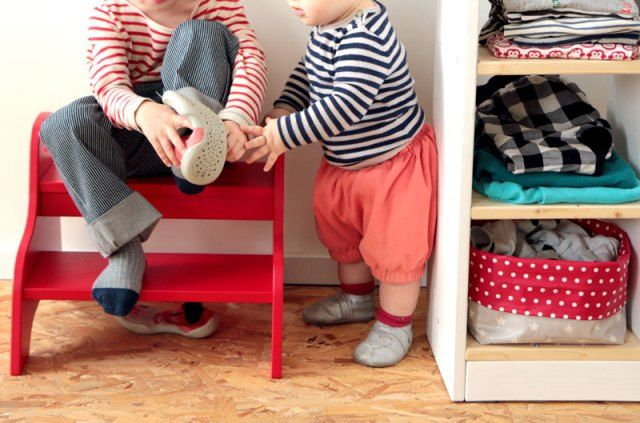
\includegraphics[scale=0.25]{shabiller.jpg}
            }
            \only<4>{
              
\includegraphics[scale=0.13]{se_coiffer.jpg} \\
              Hocus Pocus
            }
            \only<6>{
              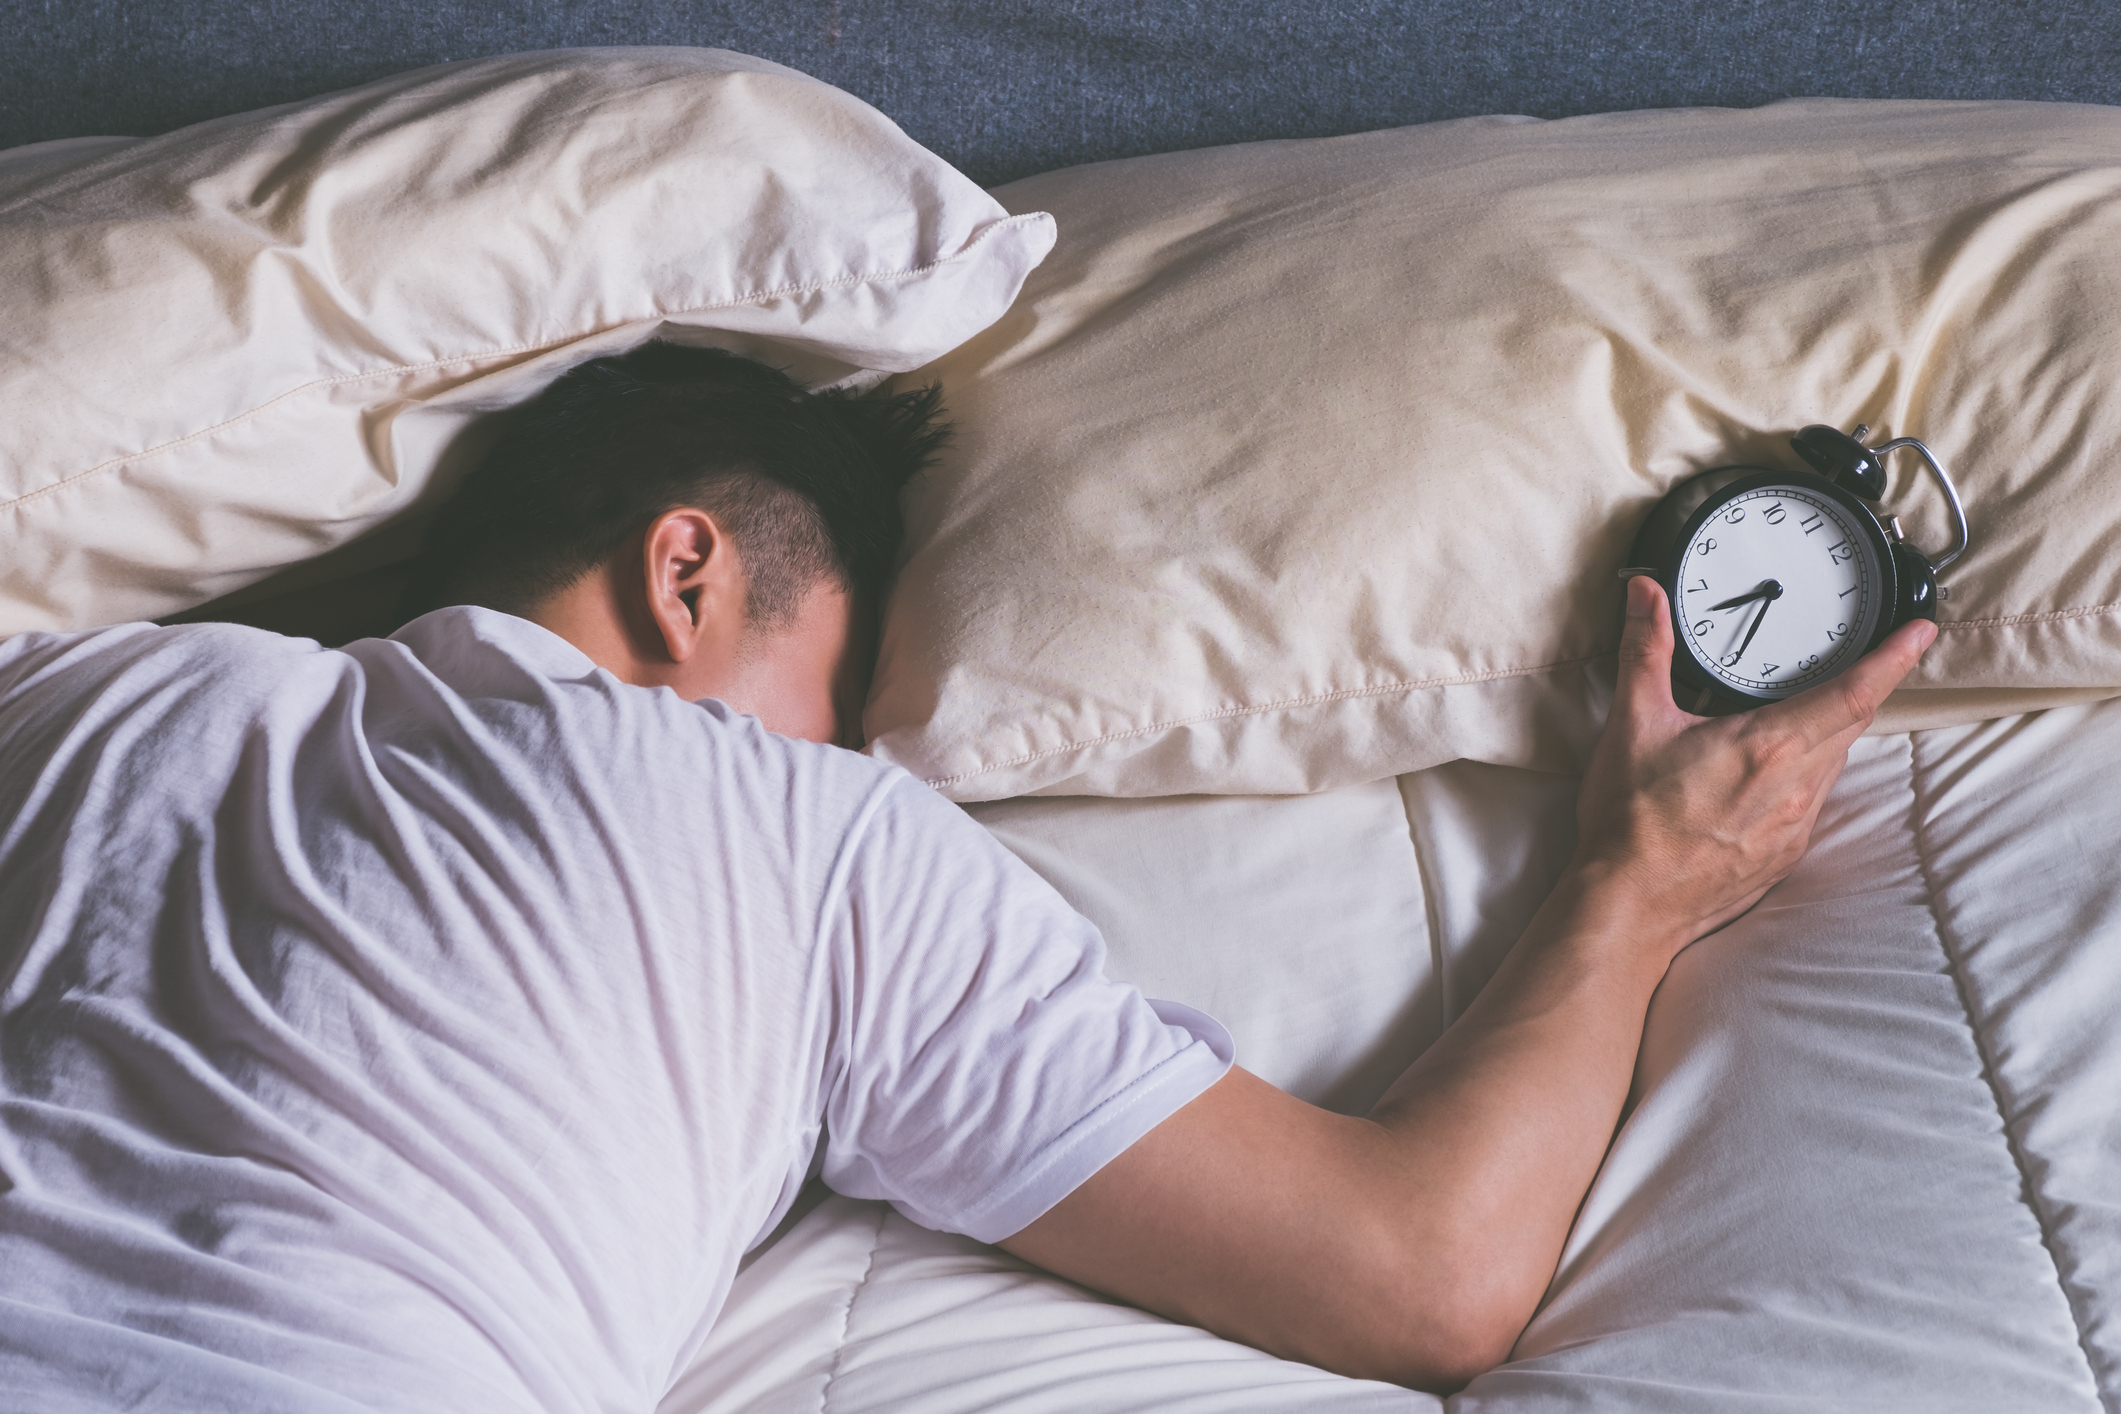
\includegraphics[scale=0.3]{se_reveiller.jpg}
            }
            \only<8>{
              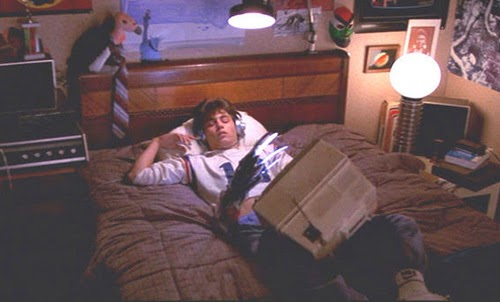
\includegraphics[scale=0.35]{freddy_lit.jpg} \\
              A Nightmare on Elm Street
            }
            \only<10>{
              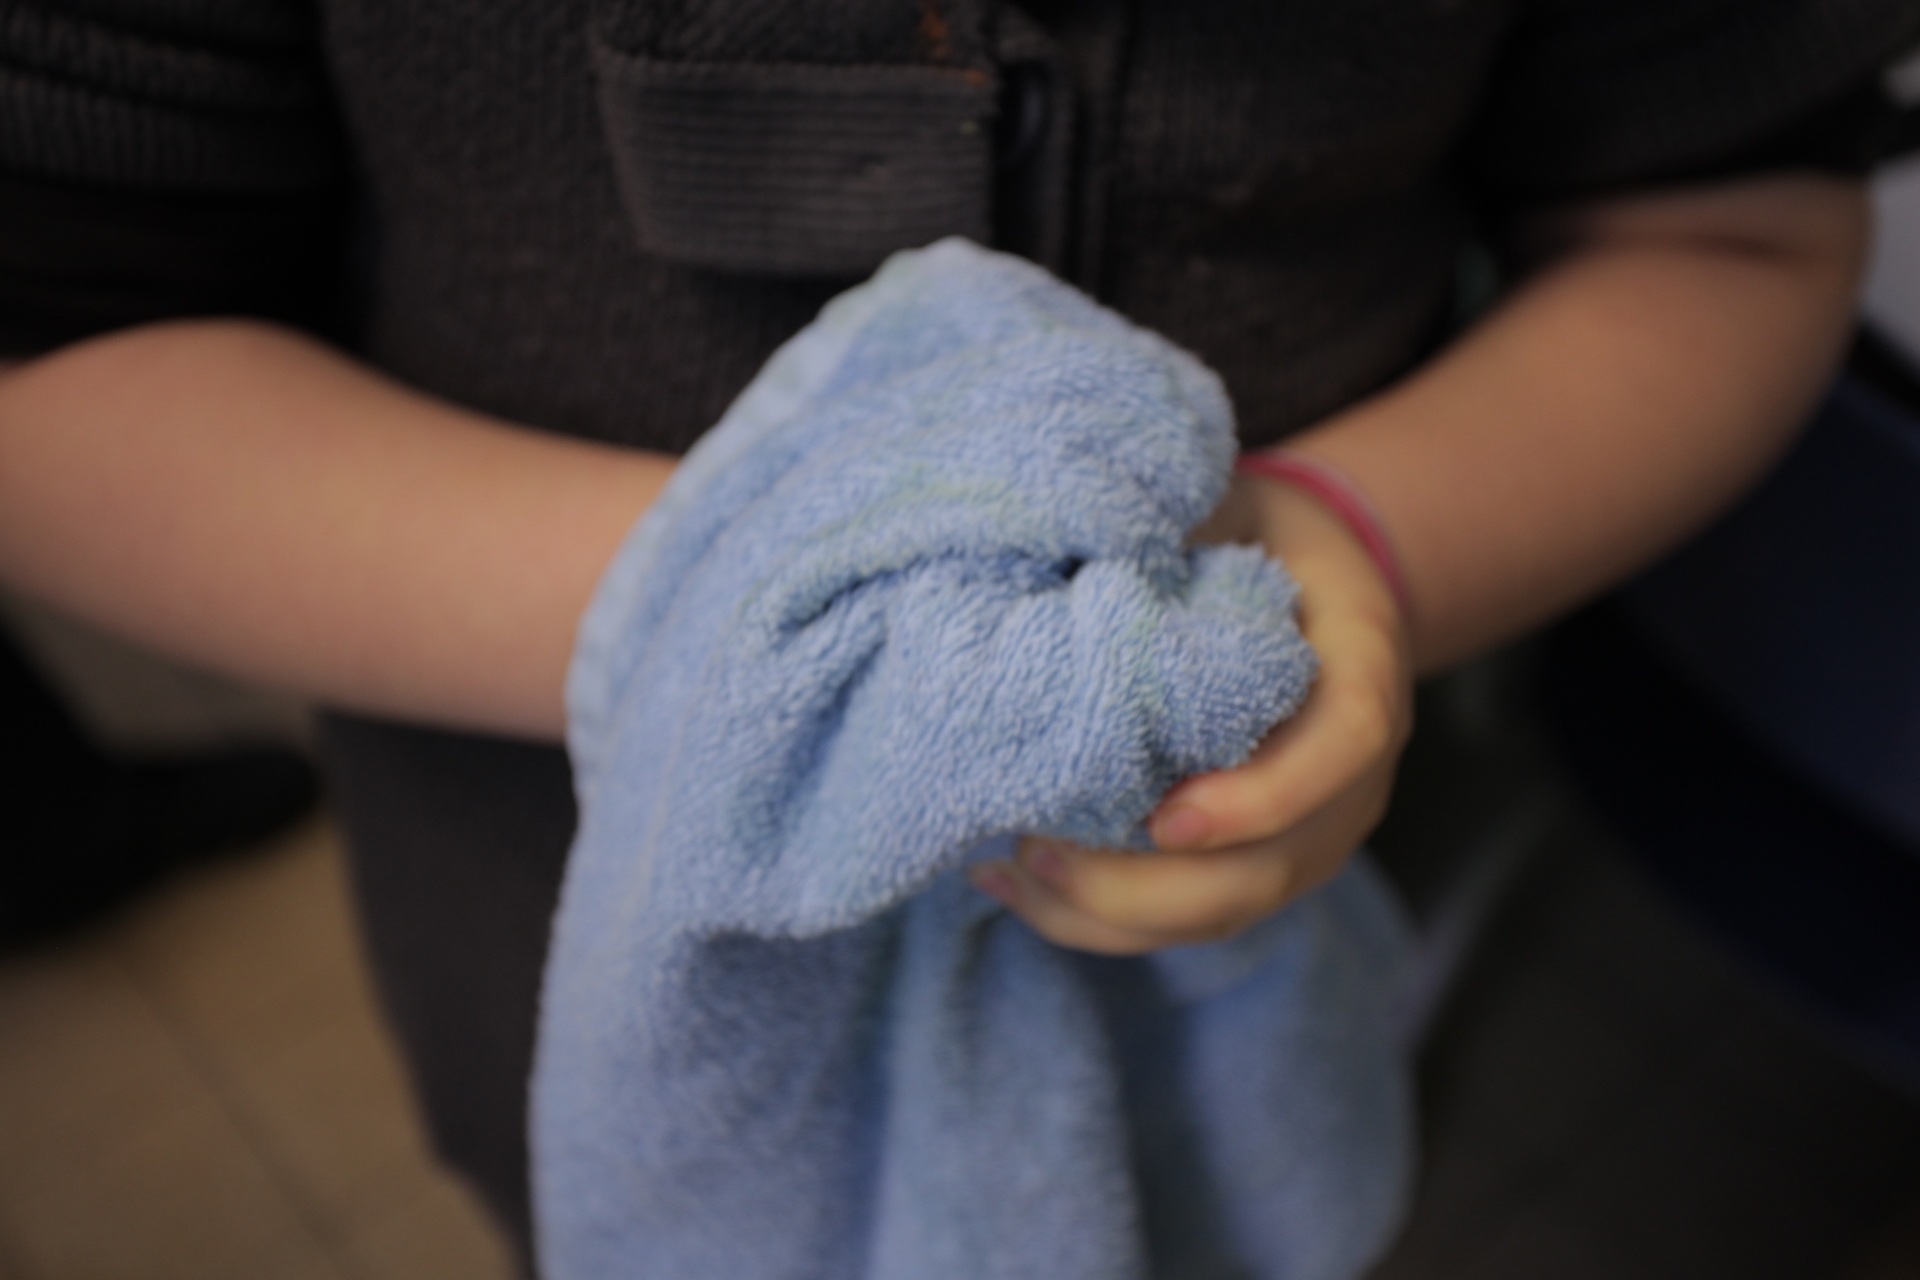
\includegraphics[scale=0.08]{sessuyer.jpg}
            }
          \end{center}
        \end{minipage}
    \end{columns}
  \end{frame}

  \begin{frame}{La matinée}
    \small
    Avec un/e partenaire, répondez aux questions suivantes, et discutez les réponses.
    \tinygloss{With a partner, answer the following questions, and discuss the answers.}
    \begin{columns}
      \scriptsize
      \column{0.4\textwidth}
        \begin{description}
          \item[] \textbf{Modèle:}
          \item[] \emph{Numéro 1}
          \item[E1:] Oui, je prends deux douches tous les jours.
          \item[] \tinygloss{Yes, I take two showers every day.}
          \item[E2:] Non, je ne prends pas deux douches tous les jours. Je prends une douche tous les deux jours.
          \item[] \tinygloss{Non, I don't take two showers every day. I take a shower every other day.}
        \end{description}
      \column{0.6\textwidth}
        Est-ce que ...
        \begin{enumerate}
          \item ... tu prends deux douches ou deux bains tous les jours?
          \item ... tu te laves les cheveux tous les jours?
          \item ... tu te brosses les dents après chaque repas \gloss{meal}?
          \item ... tu te coiffes trois ou quatre fois par jour?
          \item ... tu t'habilles différemment chaque jour?
          \item ... tu te maquilles ou tu te rases tous les jours?
          \item ... tu te mets du parfum ou de l'eau de Cologne tous les jours?
          \item ... tu te mets des bijoux \gloss{jewelry} tous les jours?
        \end{enumerate}
    \end{columns}
  \end{frame}

  \begin{frame}{Des conseils mixtes}
    \small
    En groupes de 3 ou 4, imagine les conseils que tes camarades de chambre te donneraient dans les situations suivantes, et écris-les.\\
    \tinygloss{In groups of 3 or 4, imagine the advice your roommates would give you in the following situations, and write them down.}
    \begin{columns}
      \column{0.5\textwidth}
        \begin{description}
          \item[] \textbf{Modèle:}
          \item[] \emph{Il est très tard, et tu as un examen demain.}
          \item[E1:] Alors, couche-toi!
          \item[] \tinygloss{Go to bed, then!}
          \item[E2:] Non, ne te couche pas! Continue à réviser!
          \item[] \tinygloss{No, don't go to bed! Keep reviewing!}
        \end{description}
      \column{0.5\textwidth}
        \scriptsize
        \begin{enumerate}
          \item Tu vas dîner au restaurant avec tes grands-parents.
          \item Tu as un rendez-vous avec le prof tôt ce matin.
          \item Tu as un examen important demain matin.
          \item Tu rentres du gymnase, et tu as une réunion dans dix minutes.
          \item Tu es fatigué/e, mais il est encore tôt, et tu as beaucoup de devoirs.
          \item Il est tard, mais tu as du mal à t'endormir.
        \end{enumerate}
    \end{columns}
  \end{frame}

  \begin{frame}{}
    \begin{center}
      \Large Questions?
    \end{center}
  \end{frame}
\end{document}
